% Parallel Transport on a Sphere
% Demonstrates geometric meaning of covariant derivative
% Shows path-dependence of parallel transport in curved space

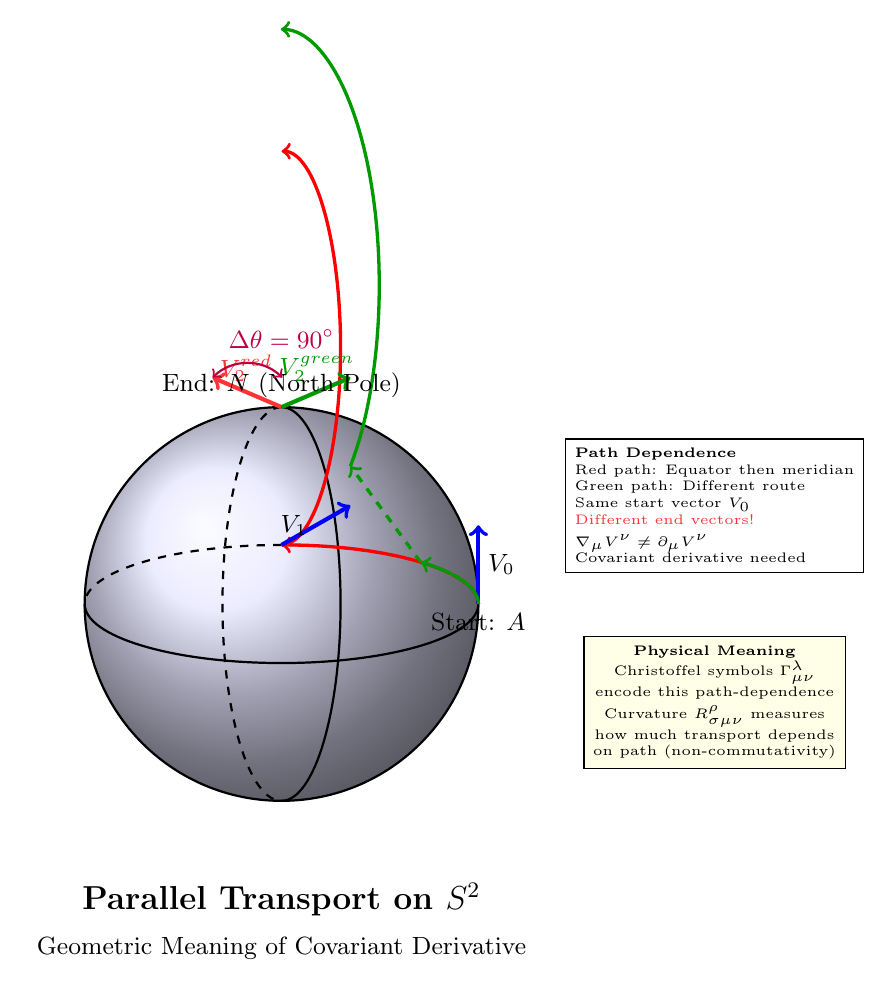
\begin{tikzpicture}[scale=2.5]

% Draw sphere
\shade[ball color=blue!10] (0,0) circle (1cm);
\draw[thick] (0,0) circle (1cm);

% Draw equator
\draw[thick, dashed] (1,0) arc (0:180:1 and 0.3);
\draw[thick] (-1,0) arc (180:360:1 and 0.3);

% Draw meridians
\draw[thick, dashed] (0,1) arc (90:270:0.3 and 1);
\draw[thick] (0,-1) arc (270:450:0.3 and 1);

% Path 1: Equator then meridian (red path)
\coordinate (A) at (1,0);
\coordinate (B) at (0,0.3);
\coordinate (C) at (0,1);

\draw[->, very thick, red] (A) arc (0:90:1 and 0.3);
\draw[->, very thick, red] (B) arc (-90:90:0.3 and 1);

% Vector at start (pointing north)
\draw[->, very thick, blue, line width=1.5pt] (1,0) -- (1,0.4);
\node[right, font=\small] at (1,0.2) {$V_0$};

% Vector after equator transport (still pointing north)
\draw[->, very thick, blue, line width=1.5pt] (0,0.3) -- (0.35,0.5);
\node[left, font=\small] at (0.18,0.4) {$V_1$};

% Vector at north pole after meridian transport (rotated!)
\draw[->, very thick, red!80, line width=1.5pt] (0,1) -- (-0.35,1.15);
\node[above, font=\small, text=red!80] at (-0.18,1.08) {$V_2^\text{red}$};

% Path 2: Different route (green path)
\draw[->, very thick, green!60!black] (A) arc (0:45:1 and 0.3);
\draw[->, very thick, green!60!black, dashed] (0.707,0.212) -- (0.35,0.7);
\draw[->, very thick, green!60!black] (0.35,0.7) arc (-45:90:0.5 and 1.3);

% Vector at north pole via green path (different rotation!)
\draw[->, very thick, green!60!black, line width=1.5pt] (0,1) -- (0.35,1.15);
\node[above, font=\small, text=green!60!black] at (0.18,1.08) {$V_2^\text{green}$};

% Labels
\node[below, font=\small] at (1,0) {Start: $A$};
\node[above, font=\small] at (0,1) {End: $N$ (North Pole)};

% Angle annotation
\draw[<->, thick, purple] (-0.35,1.15) arc (135:45:0.25);
\node[above, font=\small, text=purple] at (0,1.25) {$\Delta\theta = 90^\circ$};

% Legend box
\node[draw, fill=white, align=left, font=\tiny] at (2.2,0.5) {
    \textbf{Path Dependence}\\
    Red path: Equator then meridian\\
    Green path: Different route\\
    Same start vector $V_0$\\
    \textcolor{red!80}{Different end vectors!}\\[2pt]
    $\nabla_\mu V^\nu \neq \partial_\mu V^\nu$\\
    Covariant derivative needed
};

% Physical interpretation
\node[draw, fill=yellow!10, align=center, font=\tiny] at (2.2,-0.5) {
    \textbf{Physical Meaning}\\
    Christoffel symbols $\Gamma^\lambda_{\mu\nu}$\\
    encode this path-dependence\\[2pt]
    Curvature $R^\rho_{\sigma\mu\nu}$ measures\\
    how much transport depends\\
    on path (non-commutativity)
};

% Title
\node[font=\large\bfseries] at (0,-1.5) {Parallel Transport on $S^2$};
\node[font=\small] at (0,-1.75) {Geometric Meaning of Covariant Derivative};

\end{tikzpicture}
